\subsubsection{UC25 - Visualizzazione lista messaggi nella chat}\label{UC25}
\paragraph*{Descrizione}
L'Utente visualizza il contenuto di una chat. La lista dei messaggi comprende sia le richieste dell'Utente che le risposte del ChatBOT.

\paragraph*{Attori principali}
Utente

\paragraph*{Precondizioni}
\begin{itemize}
  \item Il sistema è attivo e funzionante;
  \item È presente almeno un messaggio nella chat.
\end{itemize}

\paragraph*{Postcondizioni}
\begin{itemize}
  \item Viene visualizzato correttamente il contenuto della chat.
\end{itemize}

\paragraph*{Trigger}
L'Utente vuole visualizzare la lista dei messaggi nella chat.

\paragraph*{Scenario principale}
\begin{enumerate}
  \item L'Utente visualizza il contenuto della chat.
\end{enumerate}

\paragraph*{Sottocasi d'uso:}
\begin{itemize}
  \item UC25.1: Visualizzazione singolo messaggio nella chat.
\end{itemize}

\begin{figure}[H]
  \centering
  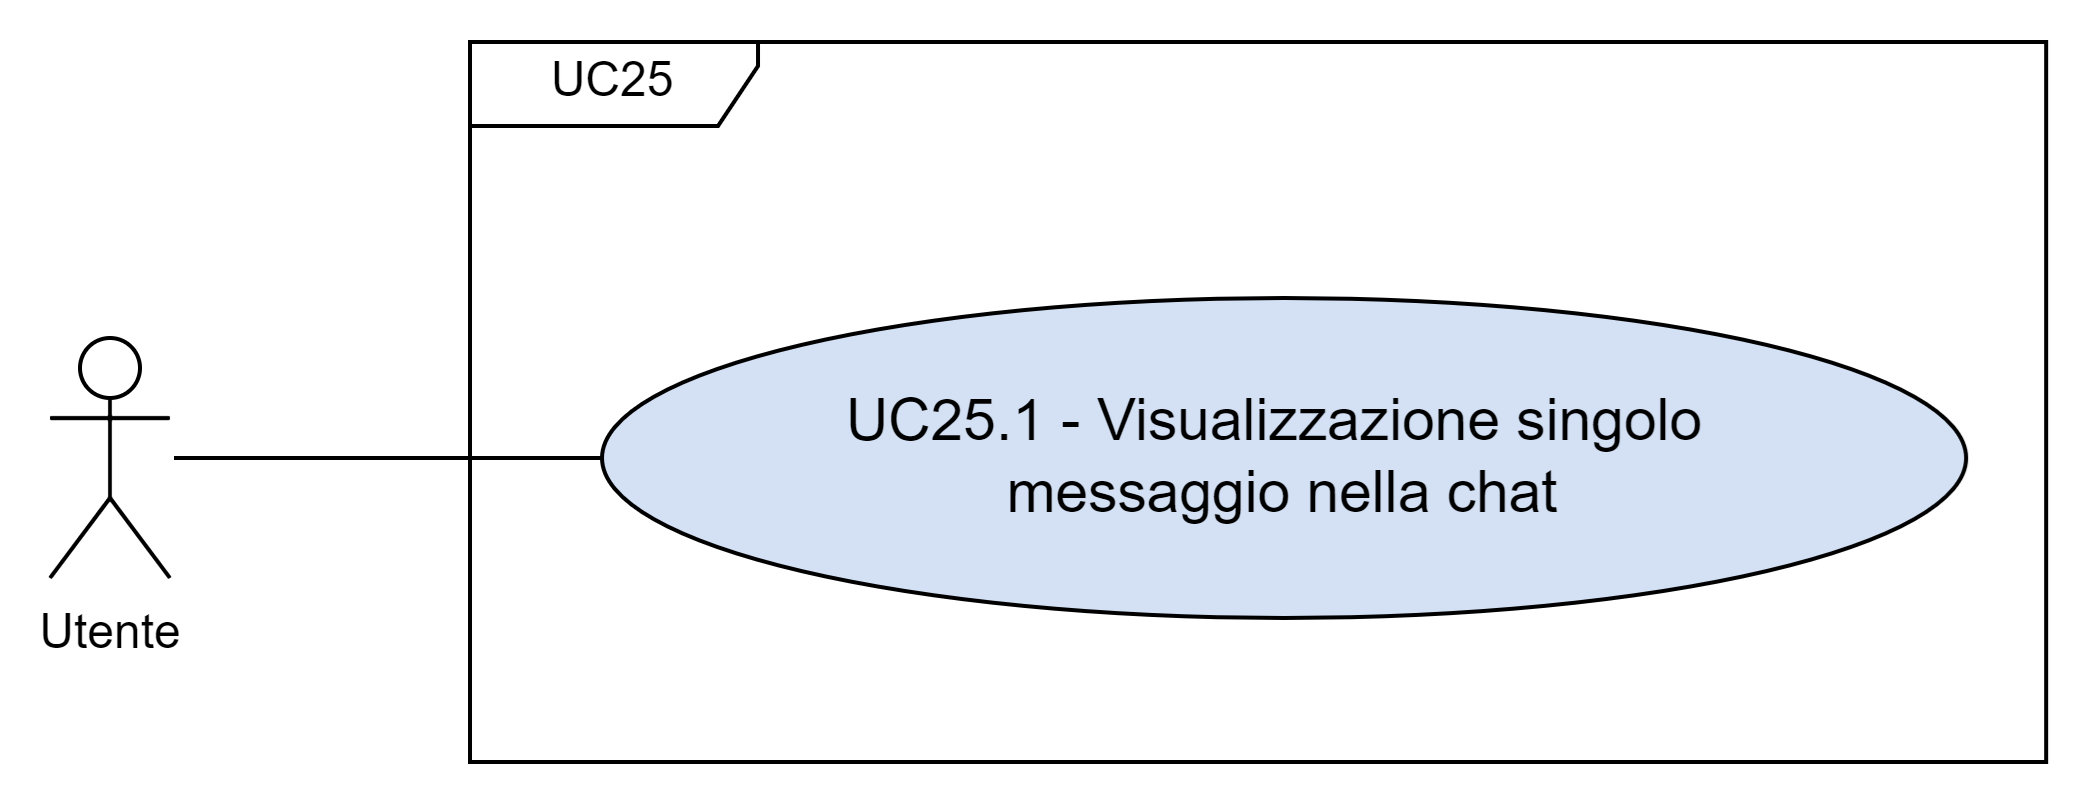
\includegraphics[width=0.90\textwidth]{assets/uc25.png}
  \caption{UC25 - Sottocasi d'uso}
\end{figure}

%%%%%%%%%%%%%%%%%%%%%%%%%%%%%%%%%%%%%%%%%%%%%%%%%%%%%%%%%%%%%%%%%%%%%%%%%%%%%%

\subsubsection{UC25.1 - Visualizzazione singolo messaggio nella chat}\label{UC25point1}
\paragraph*{Descrizione}
L'Utente visualizza un messaggio nella chat.

\paragraph*{Attori principali}
Utente

\paragraph*{Precondizioni}
\begin{itemize}
  \item L'Utente sta visualizzando la lista dei messaggi (\hyperref[UC25]{UC25}).
\end{itemize}

\paragraph*{Postcondizioni}
\begin{itemize}
  \item Il sistema mostra il singolo messaggio nella chat.
\end{itemize}

\paragraph*{Trigger}
L'Utente vuole visualizzare un singolo messaggio all'interno della chat.

\paragraph*{Scenario principale}
\begin{enumerate}
  \item L'Utente visualizza il messaggio.
\end{enumerate}

\paragraph*{Sottocasi d'uso:}
\begin{itemize}
  \item UC25.1.1: Visualizzazione contenuto messaggio;
  \item UC25.1.2: Visualizzazione mittente messaggio.
\end{itemize}

\begin{figure}[H]
  \centering
  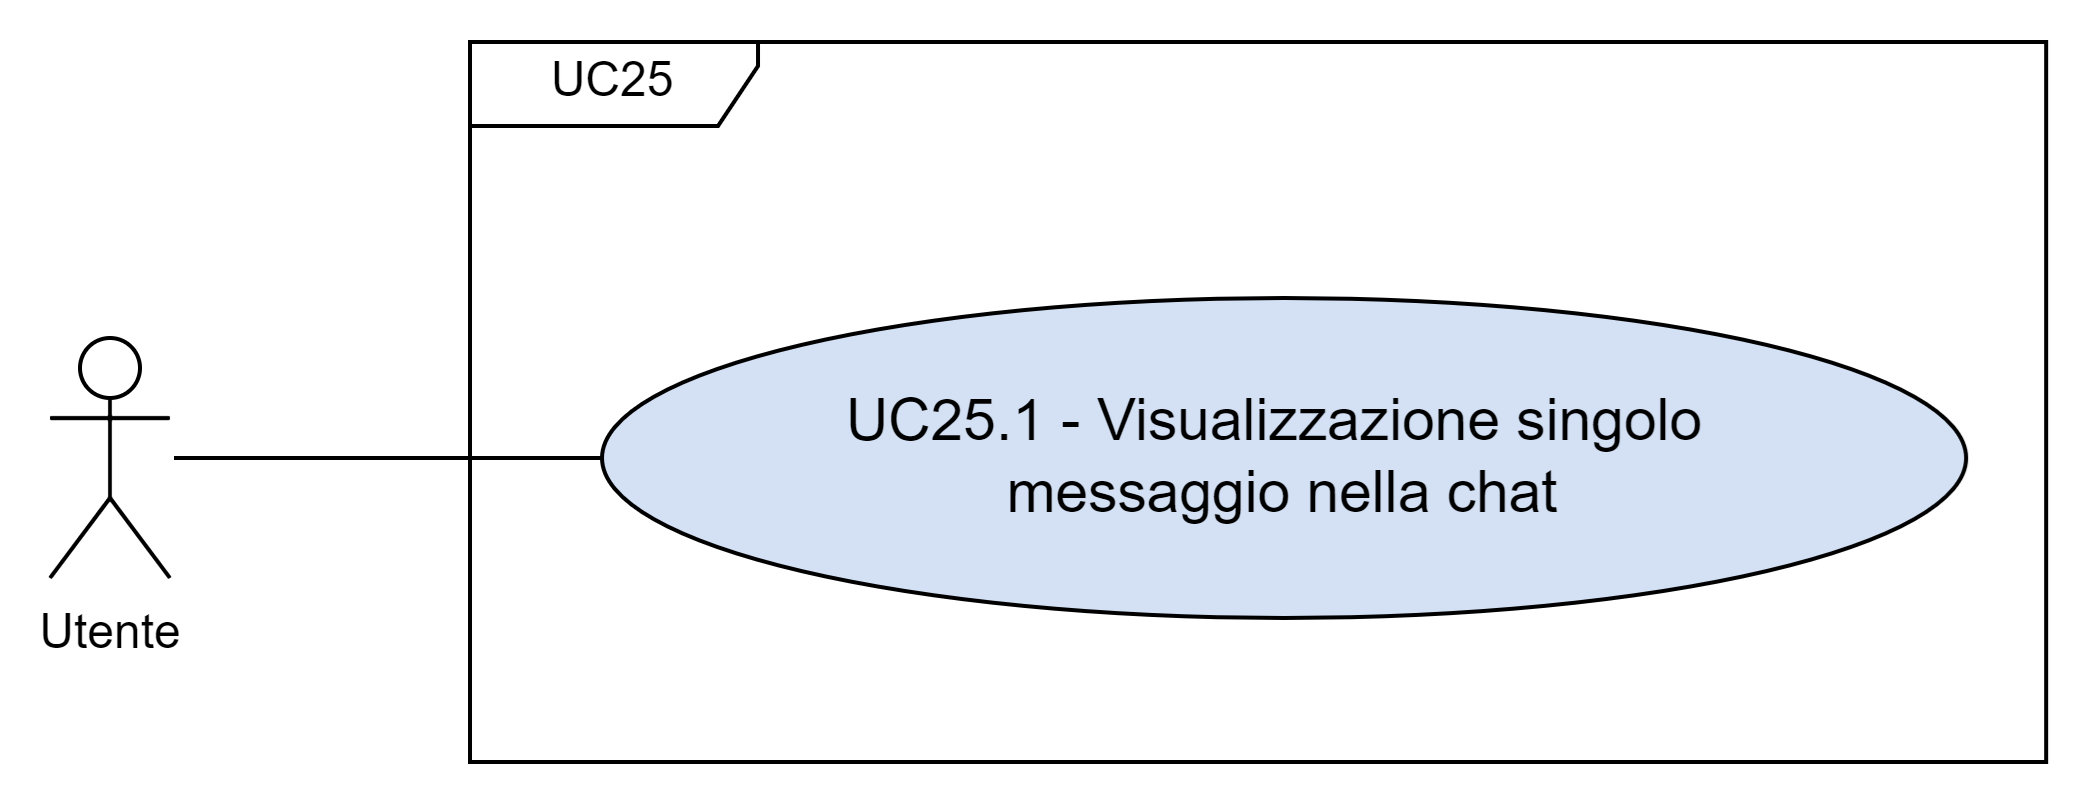
\includegraphics[width=0.90\textwidth]{assets/uc25_1.png}
  \caption{UC25.1 - Sottocasi d'uso}
\end{figure}

%%%%%%%%%%%%%%%%%%%%%%%%%%%%%%%%%%%%%%%%%%%%%%%%%%%%%%%%%%%%%%%%%%%%%%%%%%%%%%

\subsubsection{UC25.1.1 - Visualizzazione contenuto messaggio}\label{UC25point1point1}
\paragraph*{Descrizione}
L'Utente visualizza il contenuto di un messaggio. 

\paragraph*{Attori principali}
Utente

\paragraph*{Precondizioni}
\begin{itemize}
  \item L'Utente sta visualizzando un singolo messaggio nella chat (\hyperref[UC25point1]{UC25.1}).
\end{itemize}

\paragraph*{Postcondizioni}
\begin{itemize}
  \item Viene visualizzato correttamente il contenuto del messaggio.
\end{itemize}

\paragraph*{Trigger}
L'Utente vuole visualizzare il contenuto di un messaggio all'interno della chat.

\paragraph*{Scenario principale}
\begin{enumerate}
  \item L'Utente visualizza il contenuto del messaggio.
\end{enumerate}

%%%%%%%%%%%%%%%%%%%%%%%%%%%%%%%%%%%%%%%%%%%%%%%%%%%%%%%%%%%%%%%%%%%%%%%%%%%%%%

\subsubsection{UC25.1.2 - Visualizzazione mittente messaggio}\label{UC25point1point2}
\paragraph*{Descrizione}
L'Utente visualizza il mittente di un messaggio. Il mittente può essere l'Utente stesso o il ChatBOT.

\paragraph*{Attori principali}
Utente

\paragraph*{Precondizioni}
\begin{itemize}
  \item L'Utente sta visualizzando un singolo messaggio nella chat (\hyperref[UC25point1]{UC25.1}).
\end{itemize}

\paragraph*{Postcondizioni}
\begin{itemize}
  \item Viene visualizzato correttamente il mittente del messaggio.
\end{itemize}

\paragraph*{Trigger}
L'Utente vuole visualizzare il mittente di un messaggio all'interno della chat.

\paragraph*{Scenario principale}
\begin{enumerate}
  \item L'Utente visualizza il mittente del messaggio.
\end{enumerate}

